\documentclass[10pt,a4paper]{article}
\usepackage[utf8]{inputenc}
%\usepackage[french]{babel}
\usepackage{tikz-network}
\usepackage{tikz}
\usepackage{graphics,multirow}
\usepackage{subcaption}
\usepackage{array}
\usepackage{xcolor}
\PassOptionsToPackage{hyphens}{url}
\usepackage{hyperref}
\usepackage{amsmath}
\usepackage{amsfonts}
\usepackage{amssymb}
\usepackage{mathtools}
\usepackage[total={6in,8in}]{geometry}
\usepackage[backend=biber,style=numeric,sorting=ynt]{biblatex}
\addbibresource{report.bib}
 \hypersetup{
 %   bookmarks=true,         % show bookmarks bar?
 %   unicode=false,          % non-Latin characters in Acrobat’s bookmarks
 %   pdftoolbar=true,        % show Acrobat’s toolbar?
 %   pdfmenubar=true,        % show Acrobat’s menu?
 %   pdffitwindow=false,     % window fit to page when opened
 %   pdfstartview={FitH},    % fits the width of the page to the window
 %   pdftitle={My title},    % title
 %   pdfauthor={Author},     % author
 %   pdfsubject={Subject},   % subject of the document
 %   pdfcreator={Creator},   % creator of the document
 %   pdfproducer={Producer}, % producer of the document
 %   pdfkeywords={keyword1, key2, key3}, % list of keywords
 %   pdfnewwindow=true,      % links in new PDF window
    colorlinks=true,       % false: boxed links; true: colored links
    linkcolor=blue,          % color of internal links (change box color with linkbordercolor)
    citecolor=blue,        % color of links to bibliography
    filecolor=blue,         % color of file links
    urlcolor=blue        % color of external links
}
%% COLORS %%
%
\definecolor{mygreen}{RGB}{0,214,0}
%% MACROS %%

\newcommand\von{{\textsc{Von}}}
\newcommand\fon{{\textsc{Fon}}}
\newcommand\hon{{\textsc{Hon}}}
\newcommand\fston{$1^{\mathrm{st}}${\textsc{on}}}
\newcommand\nrep{N_{\mathrm{rep}}}
\newcommand\uprvec{\Pi_{\mathrm{Von}}^{\mathrm{U}}}
\newcommand\bprvec{\Pi_{\mathrm{1}}^{\mathrm{B}}}
\newcommand\hprvec{\Pi_{\mathrm{Von}}}
\newcommand\fprvec{\Pi_{\mathrm{1}}}
\newcommand\urank{K_{\mathrm{Von}}^{\mathrm{U}}}
\newcommand\brank{K_{\mathrm{1}}^{\mathrm{B}}}
\newcommand\hrank{K_{\mathrm{Von}}}
\newcommand\frank{K_{\mathrm{1}}}
\newcommand\vrank{K_{\mathrm{V}}}
\newcommand\reprank{K_{\mathrm{rep}}}
\newcommand{\red}[1]{\textcolor{red}{#1}}
\newcommand{\tbd}[1]{\textcolor{blue}{{\textbf{To do: #1}}}}
\newcommand{\ask}[1]{\textcolor{red}{{\textbf{Question: #1}}}}
\newcommand\mems{\textit{memory nodes}}
\newcommand\kin{k_{\mathrm{in}}}
\newcommand\kout{k_{\mathrm{out}}}
\newcommand\uhonpr{Unbiased HON PR}
\newcommand\honpr{HON PR}
\newcommand\pr{1stON PR}
\newcommand\bpr{1stON Biased PR}
%\author{Célestin Coquidé}
\title{Complexity and Fitness of Methylated DNA sites and RNAs in the context of Breast Cancer Tissues}
\date{\today}
\begin{document}
\maketitle
\section{Aim of the study}
Highlighting the nestedness structure of the bipartite network representing correlations between methylated DNA sited and RNAs.
\section{Methods and Data}
\subsection{Nestedness}
Nested structures appear in the nature such that in ecological and socio-economic systems. In ecological systems, for instance, there is a nested distribution of species habitats. Where as some species only live in particular locations, some others live in a large variety of environments including those particular locations [CITATION]. In the context of network theory, a perfectly nested structure is such that for any pair of node ($i,j$) with $k_{i} < k_{j}$ their respective degree (number of neighbors), the set of nodes $i$ is interacting with is included in the set of nodes $j$ is interacting with. The adjacency matrix of such a network shows a triangular shape when columns and rows are sorted accordingly to the degree ordering of respective nodes. There are many metrics (other than degrees) permitting to infer the nested structure of a given network. Nestedness can appear in unipartite and bipartite networks. In the context of economical systems, especially the world trade network seen as a country-product bipartite network, recent research shows the existence of nestedness [CITATION]. The metric used here is the fitness-complexity metric [DEFINITION] which is based on a non-linear iterative algorithm. Once rows (products) and columns (countries) are sorted in a decreasing ordering of complexity and fitness scores, the biadjacency matrix representing the products exported by the countries shows a triangular shape that is characteristic of nested structure.
\subsection{Data}
We used an open access cancer dataset from GDC Data Portal. From raw data consisting in methylated DNA and RNA's beta-values for up to 841 tumorous and normal breast tissues, we built a Matrix of Pearson Correlation Coefficients between Methylated DNA and RNA from these beta-values. A network representing the Pearson correlation coefficients between pairs (M-DNA,RNA) consists in a bipartite graph with coefficients as weight of the links. Two possibilities are considered either the correlation is positive or negative. Therefore we consider a signed bipartite graph with undirected links. Two other correlation matrices can be constructed from these beta-values, the DNA-DNA and RNA-RNA correlation matrices.

We are doing an analogy with the fitness-complexity nestedness model proposed in [citation] where DNAs and RNAs are treated as countries and products.
\section{Preliminary results}
Here is presented some preliminary results obtained by performing fitness-complexity model on a subset of the dataset. We are considering 120 RNAs and 106 DNAs and kept all Pearson correlation coefficients  such that $|\rho| < 0.4$ (this operation reduces the number of RNAs and DNAs constituting the bipartite network). The corresponding bi-adjacency matrix is presented in Fig.~\ref{fig:matrix} left panel and the one obtained by column and row swaps in Fig.~\ref{fig:matrix} right panel. We can see that both positive and negative Pearson correlations based interactions between DNAs and RNAs, from this subset, present a nested structure.
\begin{figure}
\resizebox{\columnwidth}{!}{%
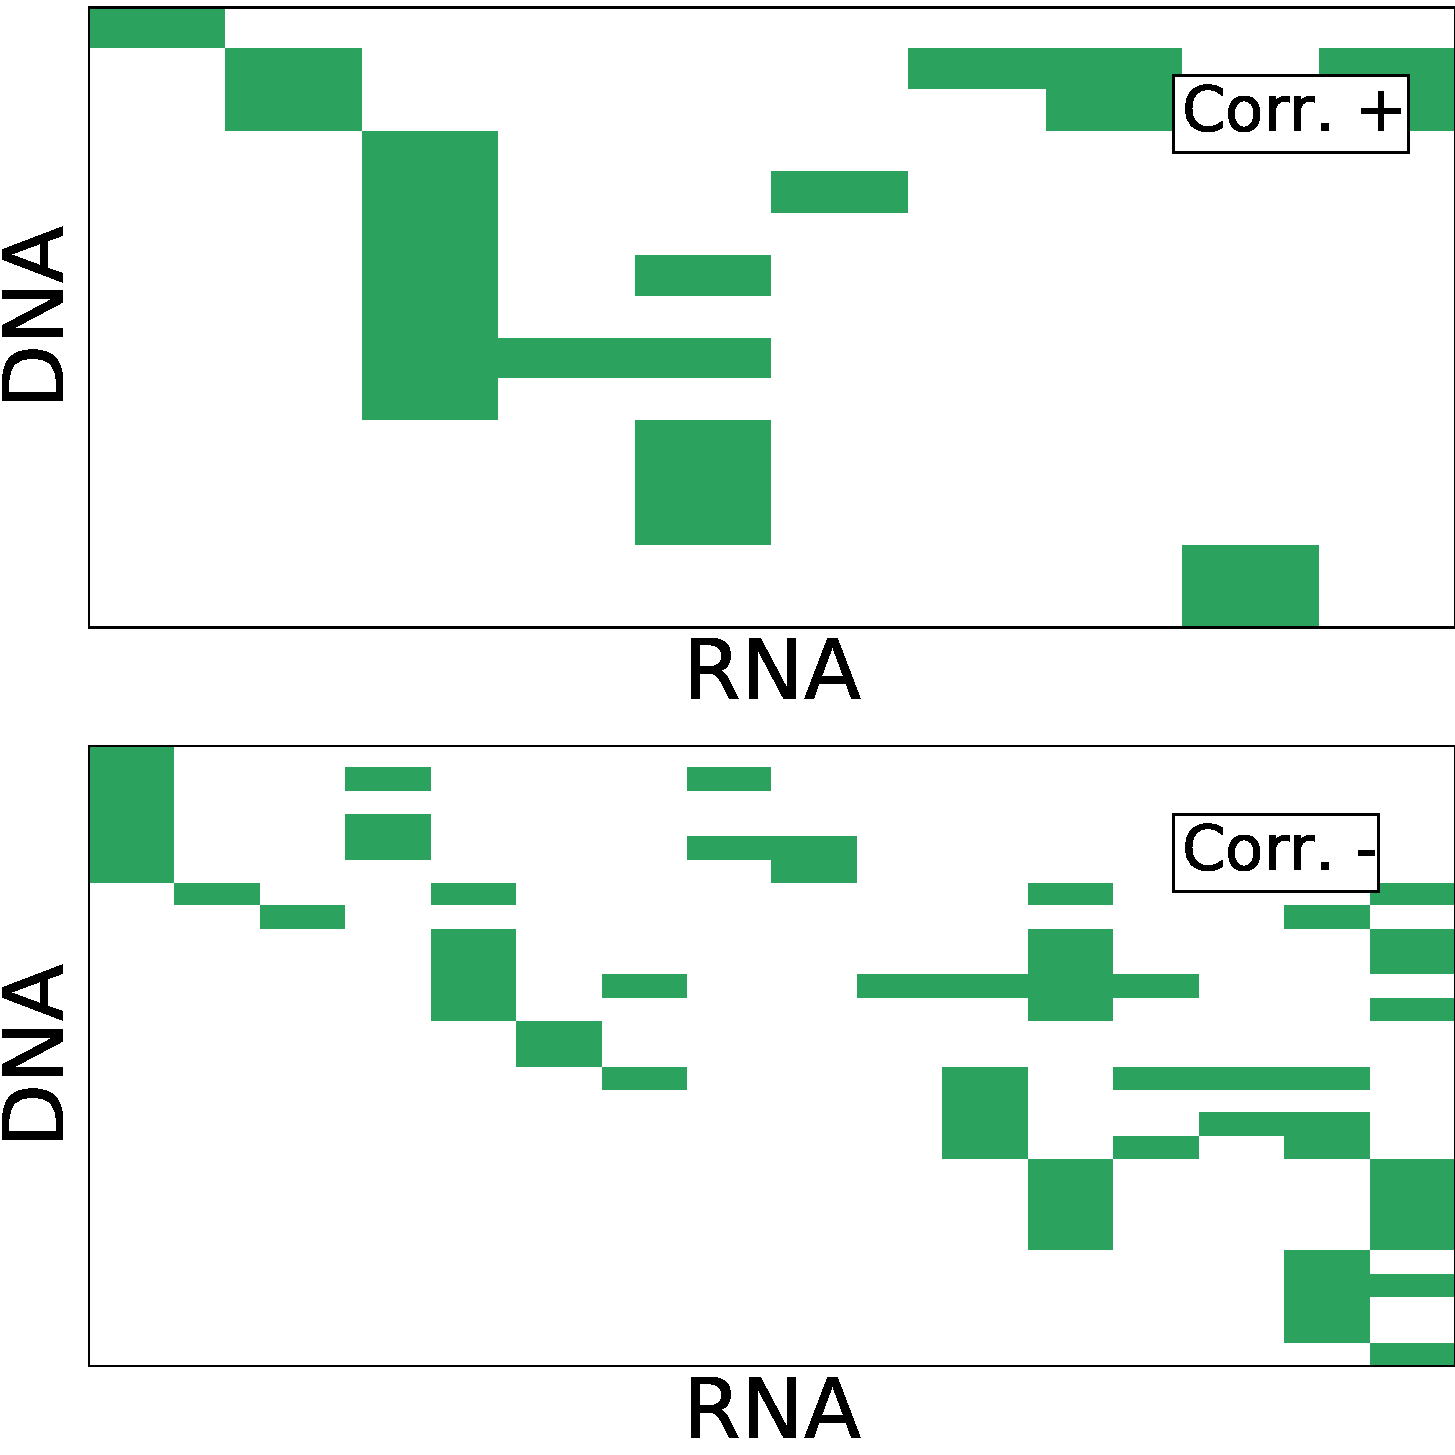
\includegraphics[width=\columnwidth]{FIG/ADN-ARN_Matrix-unit-0.4.pdf}
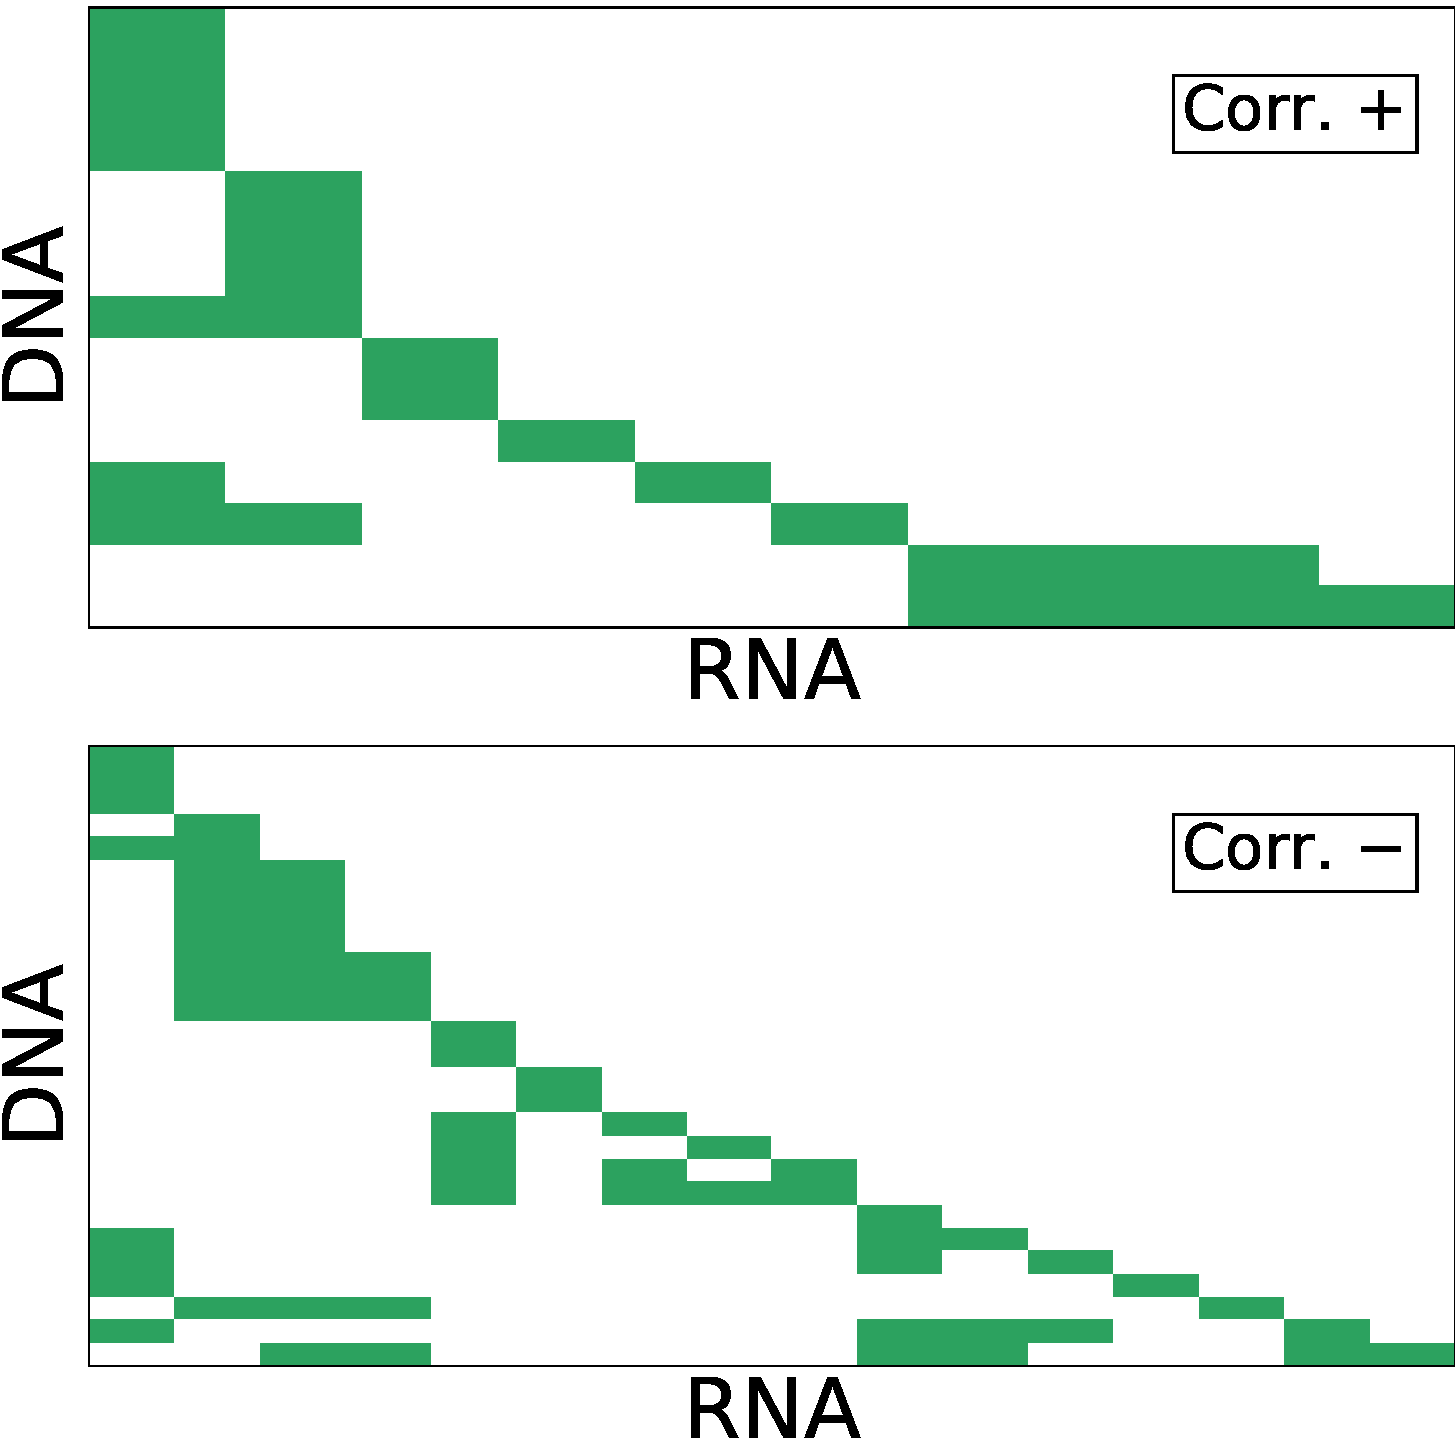
\includegraphics[width=\columnwidth]{FIG/ADN-ARN_FQ-Matrix-sum-unit-0.4.pdf}
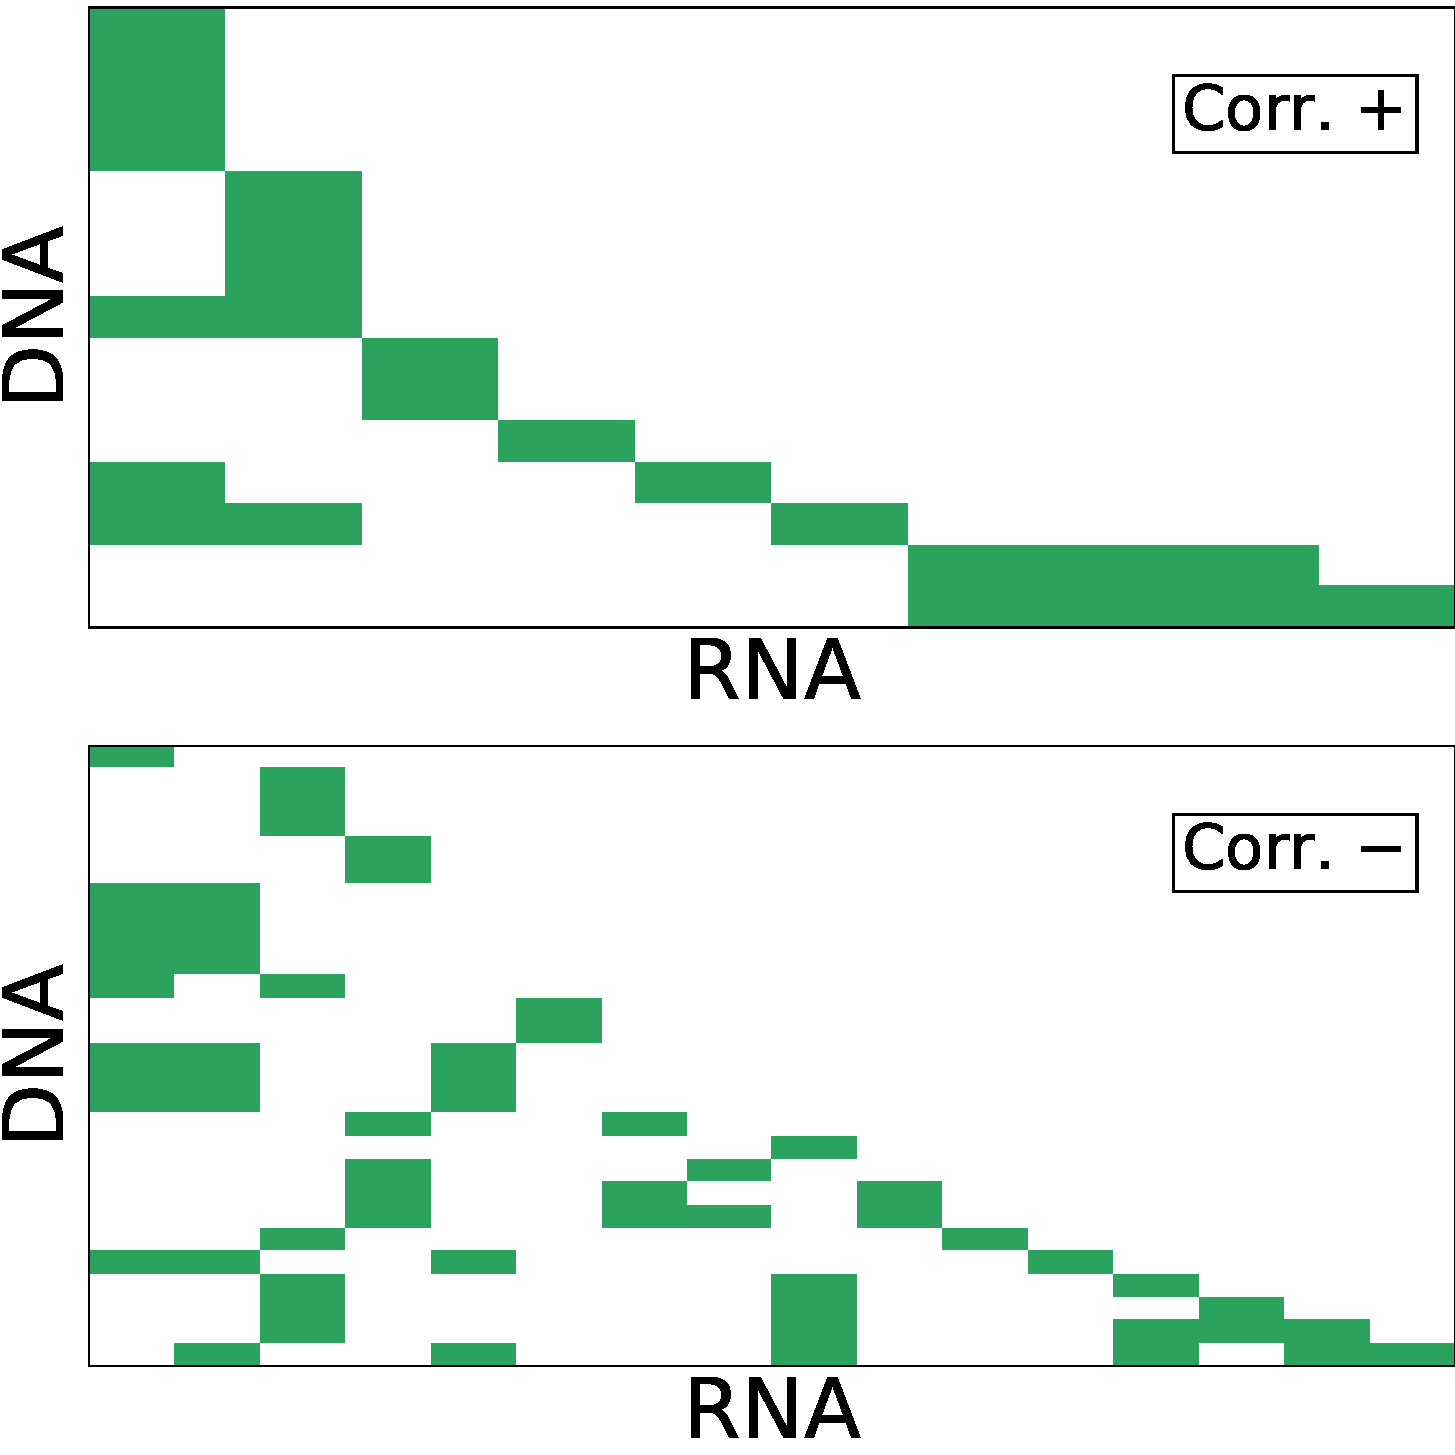
\includegraphics[width=\columnwidth]{FIG/ADN-ARN_FQ-Matrix-average-unit-0.4.pdf}
}
\caption{\label{fig:matrix}Binary bi-adjacency matrix representing the interactions between DNAs and RNAs, in the context of 841 breast tumorous tissues (left panels). Matrix entries equal $1$ (green cells) if there is an interaction between entities, $0$ otherwise (white cells). Rows (columns) have been swapped in decreasing ordering of DNAs' fitness (RNAs' complexity) scores (right panels). Positive (top panels) and negative (bottom panels) interactions have been considered independently. Pearson correlation coefficient absolute values are below $0.4$.}
\end{figure}
\printbibliography


\end{document}
